\chapter{Vision-based Position Estimator}
\label{ch:vision_based_control}

As discussed in Section \ref{sec:experiment}, the lack of precise position measurement causes the quadrotor's drift. Therefore, the quadrotor must be equipped with proper position measurement, such as a GPS sensor and a video sensor, for its stable autonomous operation. A simple and light position estimator based on image processing is introduced in this chapter. We assumed the case that the quadrotor hovers above four markers located on the floor.

This chapter consists of the following contents. First, the camera distortion model used in the system is stated. Then, the image processes used for detecting markers are described. Finally, a geometric relation between the pixel coordinates of the markers and the quadrotor's position is described, and a method to estimate the quadrotor position is introduced.

\section{Camera Calibration}
%http://www.vision.caltech.edu/bouguetj/calib_doc/htmls/parameters.html
An image from a camera is often distorted by mechanical factors; radial distortion caused by the shape of the lens, and tangential distortion caused by the angle and the distance between the video sensor and the lens. The camera used in the quadrotor system has \({120}^{\circ}\) view angle, and due to its wide angle, radial distortion is especially severe. In order to collect precise image data from the camera, calibration is required.

In this research, camera calibration is processed by GML C++ Camera Calibration Toolbox, developed by the Graphics and Media Laboratory at Moscow State University \cite{gml}. The calibration toolbox is based on the polynomial camera model. Let \( {\boldsymbol {\text x}}_d = ({\text x}_d, {\text y}_d) \) be the normalized point coordinate with distortion, and \( {\boldsymbol {\text x}} =  ({\text x}, {\text y}) \) be the normalized point coordinate without distortion. Then, the model is given as the below equation \cite{caltech_calib}.\\
\begin{equation}
\label{eq:distortion_model}
\begin{aligned}
{\text x}_d = (1 + {k_c}_1 {\text r}^2 + {k_c}_2 {\text r}^4 + {k_c}_5 {\text r}^6 ) {\boldsymbol {\text x}} + 
\begin{bmatrix}
2 {k_c}_3 {\text x} {\text y} + {k_c}_4 ({\text r}^2 + 2 {\text x}^2) \\
{k_c}_3 ({\text r}^2 + 2 {\text y}^2 + 2 {k_c}_4 {\text x} {\text y})
\end{bmatrix}
\end{aligned}
\end{equation}\\
where \({\boldsymbol k}_c = ( {k_c}_1, {k_c}_2, {k_c}_3, {k_c}_4, {k_c}_5 )\) is the distortion coefficients of the camera and \(\text r\) is defined with respect to \(\text x\) and \(\text y\) as the below equation.
\begin{equation}
\begin{aligned}
{\text r}^2 = {\text x}^2 + {\text y}^2
\end{aligned}
\end{equation}\\
In Equation (\ref{eq:distortion_model}), the first term of the right side represents radial distortion, and the second term of the right side represents tangential distortion. In addition to distortion, the pixel coordinates of the projection \(p\) is given as,
\begin{equation}
\begin{aligned}
p = K_K {\boldsymbol {\text x}}_d
\end{aligned}
\end{equation}
where \(K_K\) is the camera matrix, defined as,
\begin{equation}
\begin{aligned}
K_K = 
\begin{bmatrix}
{f_c}_1 & \alpha_c {f_c}_1 & {c_c}_1 \\
0 & {f_c}_2 & {c_c}_2 \\
0 & 0 & 1
\end{bmatrix}
\end{aligned}
\end{equation}\\
\({f_c}_1\), \({f_c}_2\) are the focal distances and \(\alpha_c\) is the angle between the x and y sensor axes. Therefore, by measuring the distortion coefficients  \( \boldsymbol{k}_c\) and the camera matrix \(K_K\), the undistorted coordinate \( \boldsymbol{\text x} \) can be restored from the raw pixel coordinate \(p\). Figure \ref{fig:camera_calibration} shows the results of the marker image restored from the raw image by camera calibration.
\begin{figure}
    \centering
    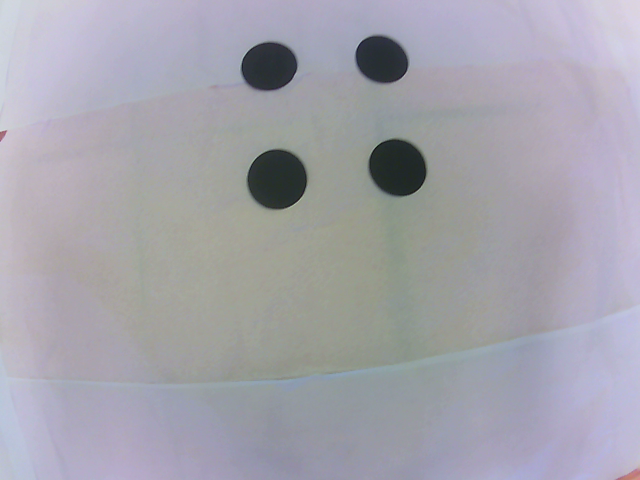
\includegraphics[width=0.45\textwidth]{graphics/raw.png}
    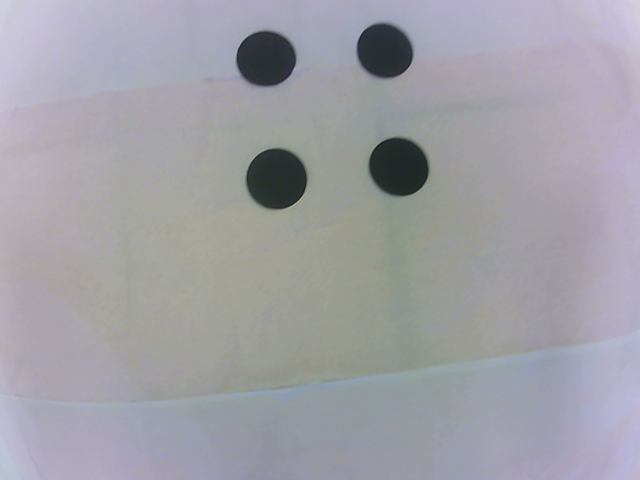
\includegraphics[width=0.45\textwidth]{graphics/undistorted.png}
    \caption{Camera Calibration (Left: Raw Image, Right: Restored Image)}
    \label{fig:camera_calibration}
\end{figure}

\section{Marker Detection}
Marker detection can be achieved by multiple image processes. First of all, a monochrome image is used. In order to decrease noise and find clear borders, the image is filtered by the Gaussian filter and thresholded. Then, the morphology closing transformation is processed to restore holes on the borders. Once the image has clean borders, the markers are detected with their contours. To be specific, the "findContours" function of OpenCV 2.4 is used for the process of finding contours \cite{opencv}.

From the above image processes, the markers of the image are detectable. However, due to environmental factors, such as lightness and floor state, empty coordinates possibly be detected as markers. Therefore, the following strategy is applied in the system. Consider the case that more than 4 coordinates \(p_i\) are detected as markers. Since the reference makers are fixed and clustered, and wrongly-detected coordinates are few, usually zero or, at most, two, markers are located close to the center of the set of candidates. By using this method, incorrect candidates are excluded easily.

The result of each step is shown in Figure \ref{fig:threshold} - \ref{fig:result}. The white circles in Figure \ref{fig:result} point the centers of the image markers.

\begin{figure}
    \centering
    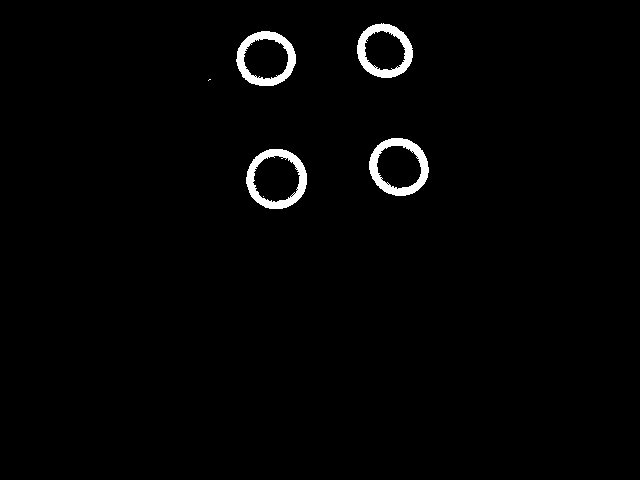
\includegraphics[width=0.45\textwidth]{graphics/threshold.png}
    \caption{Gaussian-filtered and Thresholded Image}
    \label{fig:threshold}
\end{figure}

\begin{figure}
    \centering
    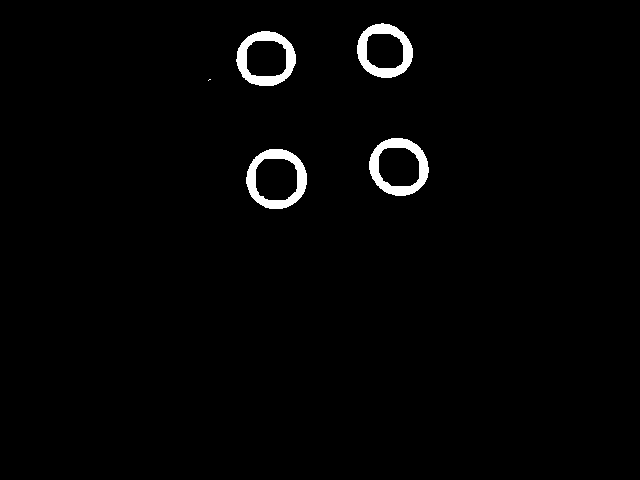
\includegraphics[width=0.45\textwidth]{graphics/contour.png}
    \caption{Restoration of Borders}
    \label{fig:contour}
\end{figure}


\begin{figure}
    \centering
    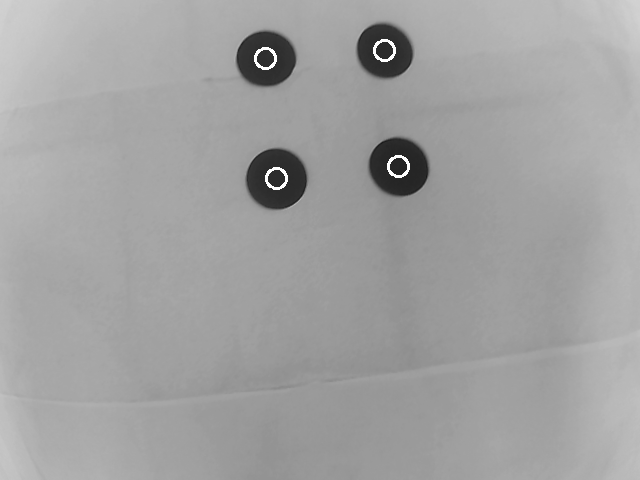
\includegraphics[width=0.45\textwidth]{graphics/result.png}
    \caption{Final Result of Marker Detection}
    \label{fig:result}
\end{figure}


\section{Position Estimation}
\begin{figure}
    \centering
    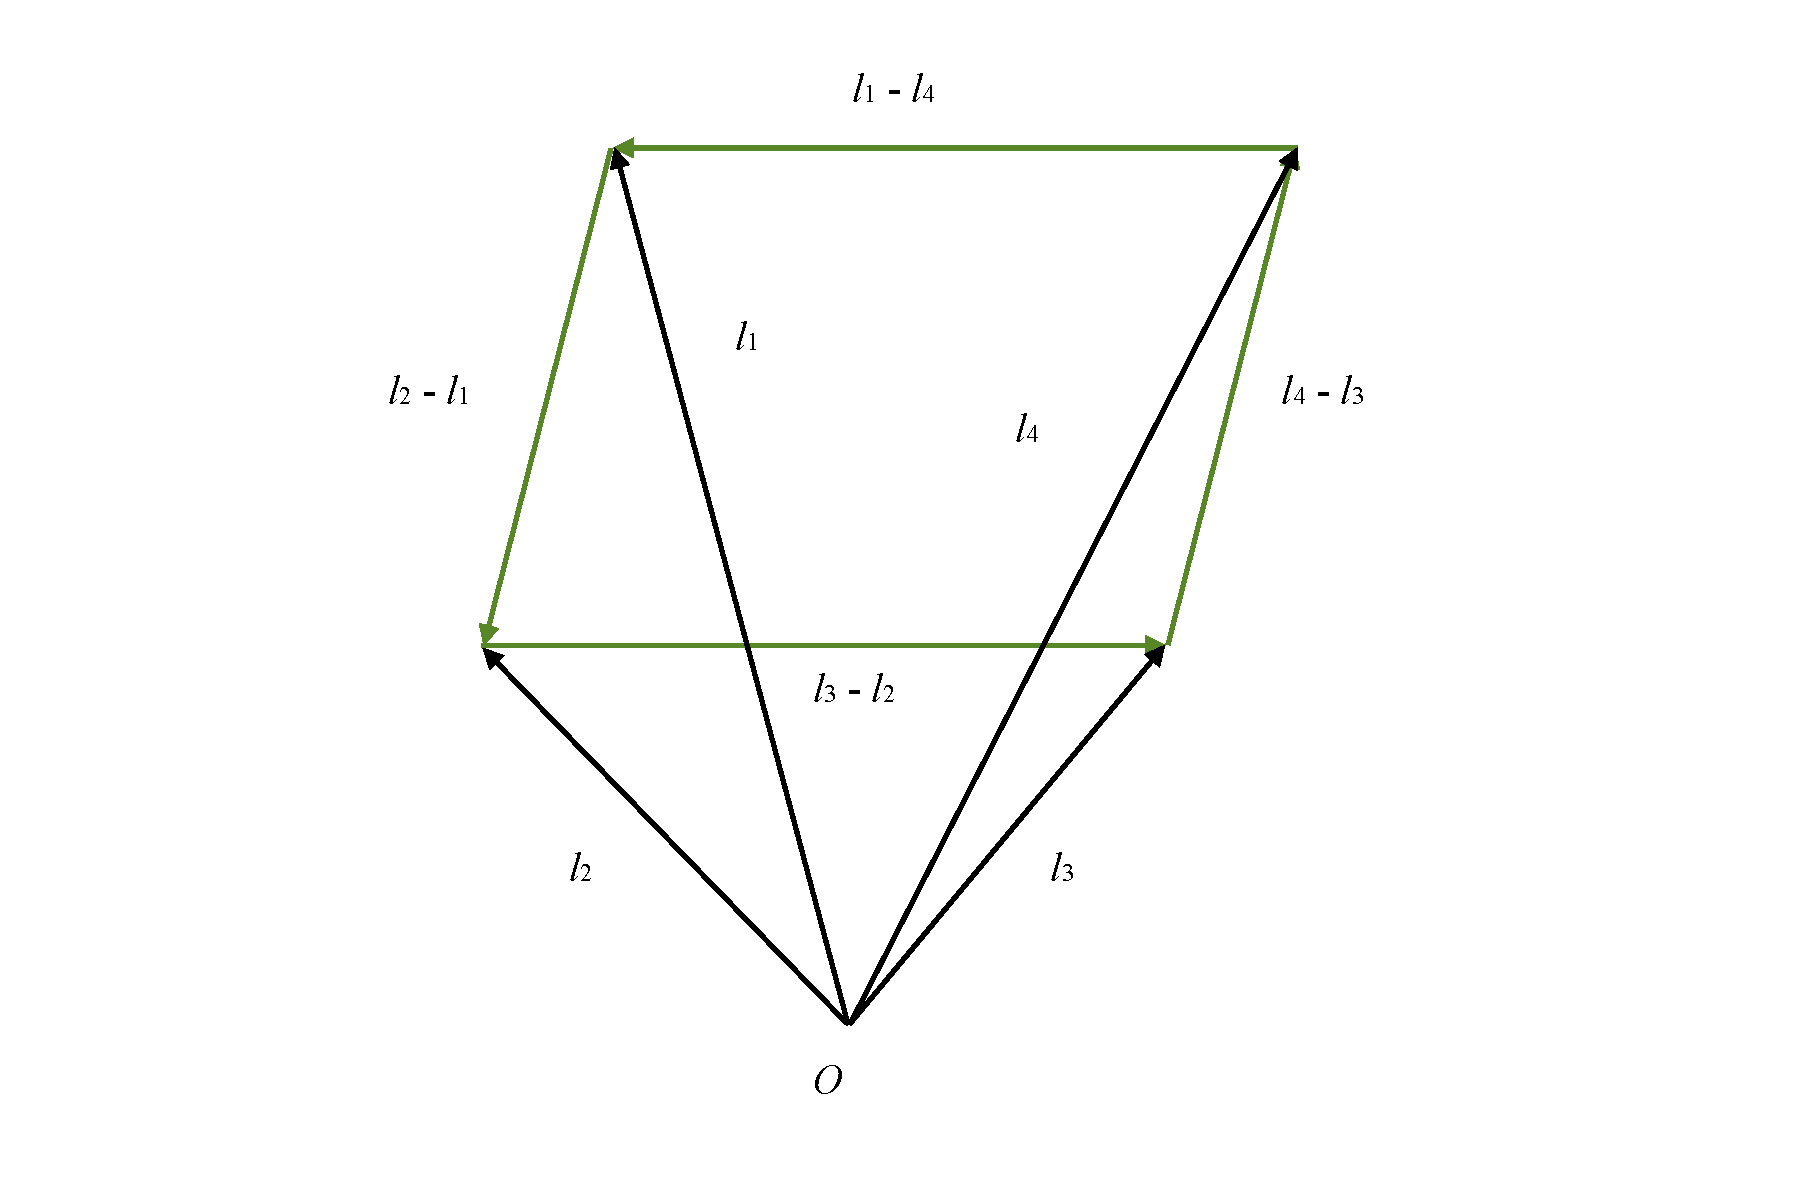
\includegraphics[width=0.8\textwidth]{graphics/scheme.pdf}
    \caption{Schematic Diagram of the Position Estimation}
    \label{fig:scheme}
\end{figure}
Let  \(\vec{ h} \) be the normal vector of the camera's orientation. Then, from Equation (\ref{eq:z_inv_eta}),  it can be represented with respect to the quadrotor's attitude \( {\boldsymbol \eta} \) as,
\begin{equation}
\begin{aligned}
{\vec h} ( {\boldsymbol \eta} ) & =  Z^{-1} 
\begin{bmatrix}
0 \\
0 \\
-1
\end{bmatrix}
 = 
\begin{bmatrix}
\sin{\theta} \\
- \sin{\phi} \cos{\theta} \\
- \cos{\phi} \cos{\theta}
\end{bmatrix}\\
\end{aligned}
\end{equation}
Let \( \boldsymbol A \) be the area of the polygon in the inertial frame, and \(\vec{l_i} \) be the relative position of a marker according to the position of the camera. Then, the projection of  \(\boldsymbol A \) is represented as below equation \cite{Haralick94}. \\
\begin{equation}
\label{eq:projection}
\begin{aligned}
{\vec h} \cdot { \boldsymbol A} & = {1 \over 2}(\vec{l_2} - \vec{l_1}) \times (\vec{l_4} - \vec{l_1}) + {1 \over 2}(\vec{l_4} - \vec{l_3}) \times (\vec{l_2} - \vec{l_3}) \\
& = {1 \over 2}(\vec{l_1} \times \vec{l_2} + \vec{l_2} \times \vec{l_3}  + \vec{l_3} \times \vec{l_4} + \vec{l_4} \times  \vec{l_1}) 
\end{aligned}
\end{equation}
From perspective projection of the camera, the relative position \(\vec{l_i}\) is represented with respect to the normalized pixel coordinate \( {\boldsymbol p}_i\), \\
\begin{equation}
\begin{aligned}
\vec{l_i} =  {d\over {\vec{h} \cdot ({R_{\psi}}^{-1} {\boldsymbol p}_i}) } {R_{\psi}}^{-1} {\boldsymbol p}_i 
\end{aligned}
\end{equation}
where \( d \) is the perpendicular distance from the camera to the plane of the markers, and it is unknown. For convenience of computation, define the composite coordinate,\\
\begin{equation}
\begin{aligned}
{{\boldsymbol p}_{\psi}}_i = {R_{\psi}}^{-1} {\boldsymbol p}_i 
\end{aligned}
\end{equation}
Then, Equation (\ref{eq:projection}) can be written as, \\
\begin{equation}
\begin{aligned}
{\vec h} \cdot { \boldsymbol A} & = {{ \Gamma d} \over 2} 
\end{aligned}
\end{equation}
where \(\Gamma \) is a composite value defined as,\\
\begin{equation}
\begin{aligned}
\Gamma = 
\left(
{{{{{\boldsymbol p}_{\psi}}_1} \times {{{\boldsymbol p}_{\psi}}_2}} \over {({\vec{h} \cdot {{\boldsymbol p}_{\psi}}_1})({\vec{h} \cdot {{\boldsymbol p}_{\psi}}_2})}} + 
{{{{{\boldsymbol p}_{\psi}}_2} \times {{{\boldsymbol p}_{\psi}}_3}} \over {({\vec{h} \cdot {{\boldsymbol p}_{\psi}}_2})({\vec{h} \cdot {{\boldsymbol p}_{\psi}}_3})}} +
{{{{{\boldsymbol p}_{\psi}}_3} \times {{{\boldsymbol p}_{\psi}}_4}} \over {({\vec{h} \cdot {{\boldsymbol p}_{\psi}}_3})({\vec{h} \cdot {{\boldsymbol p}_{\psi}}_4})}} +
{{{{{\boldsymbol p}_{\psi}}_4} \times {{{\boldsymbol p}_{\psi}}_1}} \over {({\vec{h} \cdot {{\boldsymbol p}_{\psi}}_4})({\vec{h} \cdot {{\boldsymbol p}_{\psi}}_1})}} \right) 
\end{aligned}
\end{equation}
From the above equation, \( d \) is computed as,\\
\begin{equation}
\begin{aligned}
{d} = \sqrt{{2 {\vec h} \cdot { \boldsymbol A} }\over{\Gamma}} 
\end{aligned}
\end{equation}
and therefore, the relative position of the camera according to the markers' center is given as, \\
\begin{equation}
\label{eq:relative_position}
\begin{aligned}
{\tilde {\boldsymbol r}}
& = - {1\over 4} (\vec{l_1} + \vec{l_2} + \vec{l_3} + \vec{l_4}) \\
& =  - {d \over 4} \left( { {{{\boldsymbol p}_{\psi}}_1}\over {\vec{h} \cdot {{\boldsymbol p}_{\psi}}_1} }+ { {{{\boldsymbol p}_{\psi}}_2}\over {\vec{h} \cdot {{\boldsymbol p}_{\psi}}_2} } + { {{{\boldsymbol p}_{\psi}}_3}\over {\vec{h} \cdot {{\boldsymbol p}_{\psi}}_3} } +{ {{{\boldsymbol p}_{\psi}}_4}\over {\vec{h} \cdot {{\boldsymbol p}_{\psi}}_4} } \right)
\end{aligned}
\end{equation}

Since the relative position calculated from the markers is noisy, the Kalman filter is applied to estimate and correct the value. A value computed by Equation (\ref{eq:relative_position}) passes through the Kalman filter, and the filtered value is used as relative position of the quadrotor, corresponding to the markers.

\section{Evaluation Experiment}
\subsection{Experimental Setup}
The vision-based position estimator was tested by experiments. The experiments ware also executed at the IRL motion capture arena. The quadrotor was not armed, and the autopilot only publishes the sensor values to the onboard companion computer via UART. The algorithm was run by the companion computer in real-time. In order to evaluate the results, the Vicon motion capture system of the arena was used, and streaming data from the position estimator and the motion capture system are compared. As described at Section \ref{sec:experiment}, the Vicon system detects the reflective markers on the quadrotor and measures the position of the quadrotor in its own coordinate system. The image markers used in the experiment for the position estimation are shown in Figure \ref{fig:markers}. Each image marker is a 15cm-diameter-circle and its center is located about 45 cm away from the ones of its neighbors. The placement of the image markers forms a square. The origin of the inertial coordinate system is set to be at the center of the image markers.

\begin{figure}
    \centering
    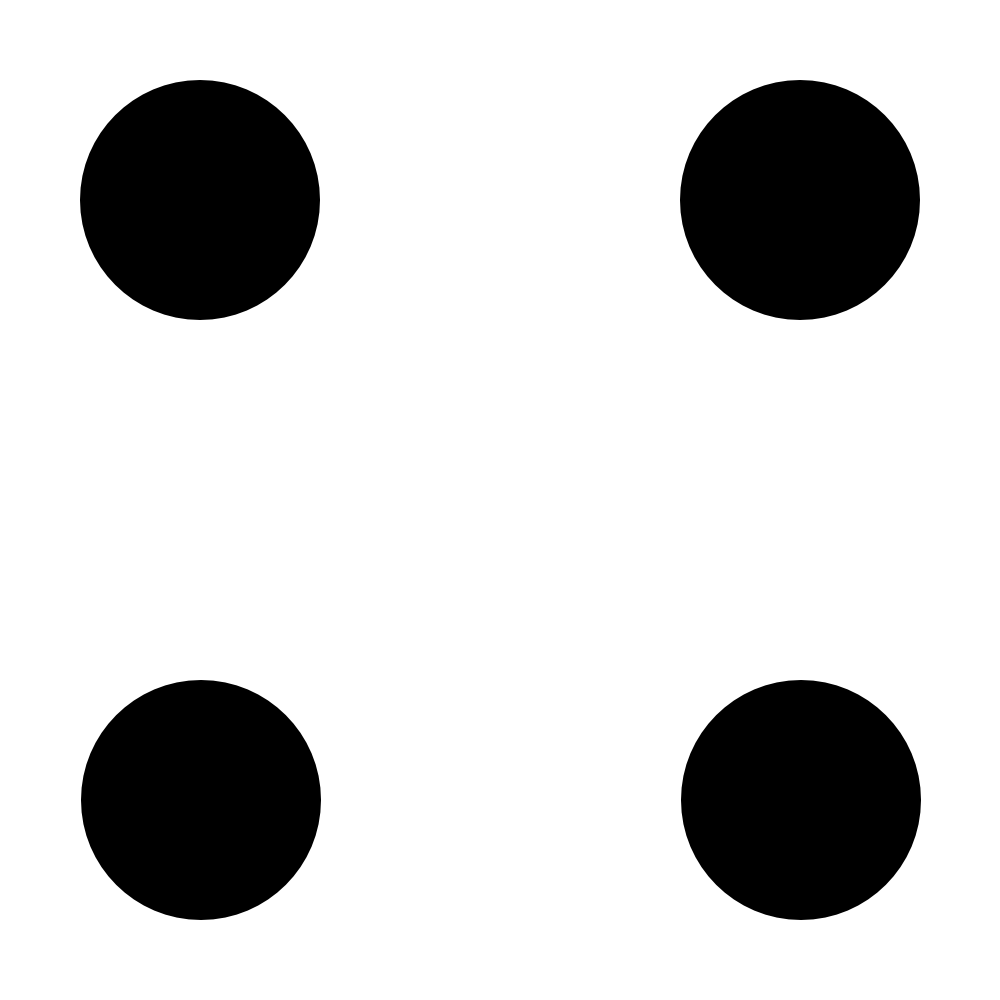
\includegraphics[width=0.45\textwidth]{graphics/markers.png}
    \caption{Image Markers for the Evaluation}
    \label{fig:markers}
\end{figure}

\subsection{Results}
All the position data from the motion capture system are filtered by a low-pass filter and transformed into the coordinate system defined by the motion capture system. The position data from the position estimator were processed by a real-time Kalman filter. The results of the experiments are shown in Figures \ref{fig:cam_x} - \ref{fig:cam_z}. Each figure shows the position measurements of both the above vision-based position estimator and the motion capture system.

\begin{figure}
    \centering
    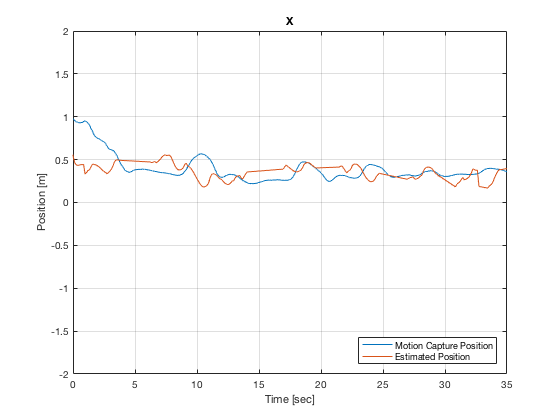
\includegraphics[width=0.45\textwidth]{graphics/cam_x.png}
    \caption{Experiment Result of the Position Estimator (x-axis Position)}
    \label{fig:cam_x}
    \vspace{1cm}
    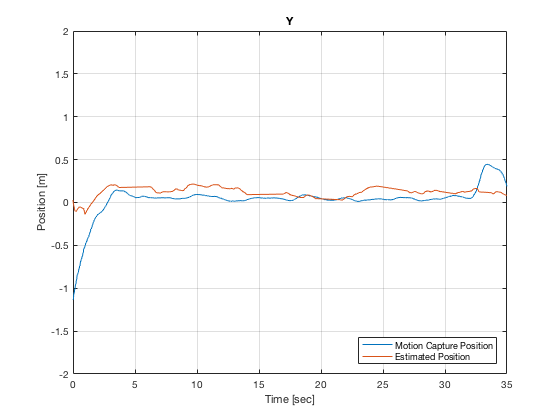
\includegraphics[width=0.45\textwidth]{graphics/cam_y.png}
    \caption{Experiment Result of the Position Estimator (y-axis Position)}
    \label{fig:cam_y}
    \vspace{1cm} 
    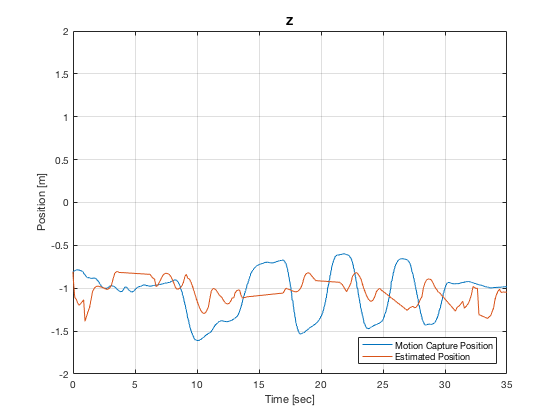
\includegraphics[width=0.45\textwidth]{graphics/cam_z.png}
    \caption{Experiment Result of the Position Estimator (z-axis Position)}
    \label{fig:cam_z}
\end{figure}

\subsection{Discussion}
As shown in Figure \ref{fig:cam_x} - \ref{fig:cam_z}, the errors of the position estimator are about 0.3 m when the position of camera moves slowly. Therefore, it can be concluded that the position estimator works roughly correctly. Considering the experimental results of x, y-axis position errors at Subsection \ref{sec:experiment} are up to 3 m and the errors grow as time pasts, the vision-based estimator is expected to improve the quadrotor's navigation.

However, as Figure \ref{fig:cam_z} shows, the position estimator is not able to reflect small change of the position among z-axis less than 0.5 m. Therefore, the position estimator is more suitable for slow flight, rather than agile performance. In addition, the camera may not capture the image markers if the camera is too close to the ground. The absence of the markers on the image frame can be a critical reason of the failure of position estimation. The problem potentially happens when the quadrotor has high roll or pitch angle, and therefore, it necessary to develop a system that deals with temporary failure of marker detection. 